\subsection{Merging of Datasets}
Following curation of individual datasets, these will need to be merged to homogenise variant calls across all data, and generate a non-sparse matrix of variant calls, where the union of variants across all samples is available for each population. This process is similar to the merger of reference panels by imputation (Figure \ref{fig:merging_reference_panels}), which could have been used, if raw reads had not been available for all populations. In order to fill the sparse matrix a union set of calls will be generated for variants that have passed filtering in each dataset (Figure \ref{fig:calling}). Prior to merging we recode any haploid male genotypes (non-PAR X and Y) to homozygous diploid genotypes if necessary. %Prior to merging 1) indels will be left aligned (e.g. bcftools norm) and 2) SNPs and indels called in low coverage data by UnifiedGenotyper will be merged into single records with bcftools (bcftools norm -m +any).
%and 3) variants called from reads aligned to build 38 will be lifted over to build 37 (liftOver). %http://hgdownload.soe.ucsc.edu/admin/exe/linux.x86_64/liftOver
Variants will be merged across cohorts (GATK CombineVariants --minimalVCF or bcftools merge | bcftools view -G). These sites will then be recalled in each dataset to generate genotype likelihoods at these sites. Sample NA12878 will not be part of the recalling and NA12878 singletons will not be called.
%Where necessary the union set of sites will be lifted over to build 38 prior to recalling and the recalled variants will then be lifted back over to build 37.
UG (--genotyping\_mode GENOTYPE\_GIVEN\_ALLELES and --output\_mode EMIT\_ALL\_SITES) will be used for recalling low coverage data.
%http://gatkforums.broadinstitute.org/discussion/4936/not-all-sites-emitted-with-genotype-given-alleles
The maximum number of allowed alternate alleles will be increased from the default 6 by multiplication with the number of original cohorts to allow all true variants to be called. Although it should only be necessary for HaplotypeCaller, interval padding will be added to ensure all known sites are called (--interval\_padding 100).
%http://gatkforums.broadinstitute.org/discussion/comment/18353
Following this, genotype refinement will be carried out.

\begin{figure}[!htbp]
\centering
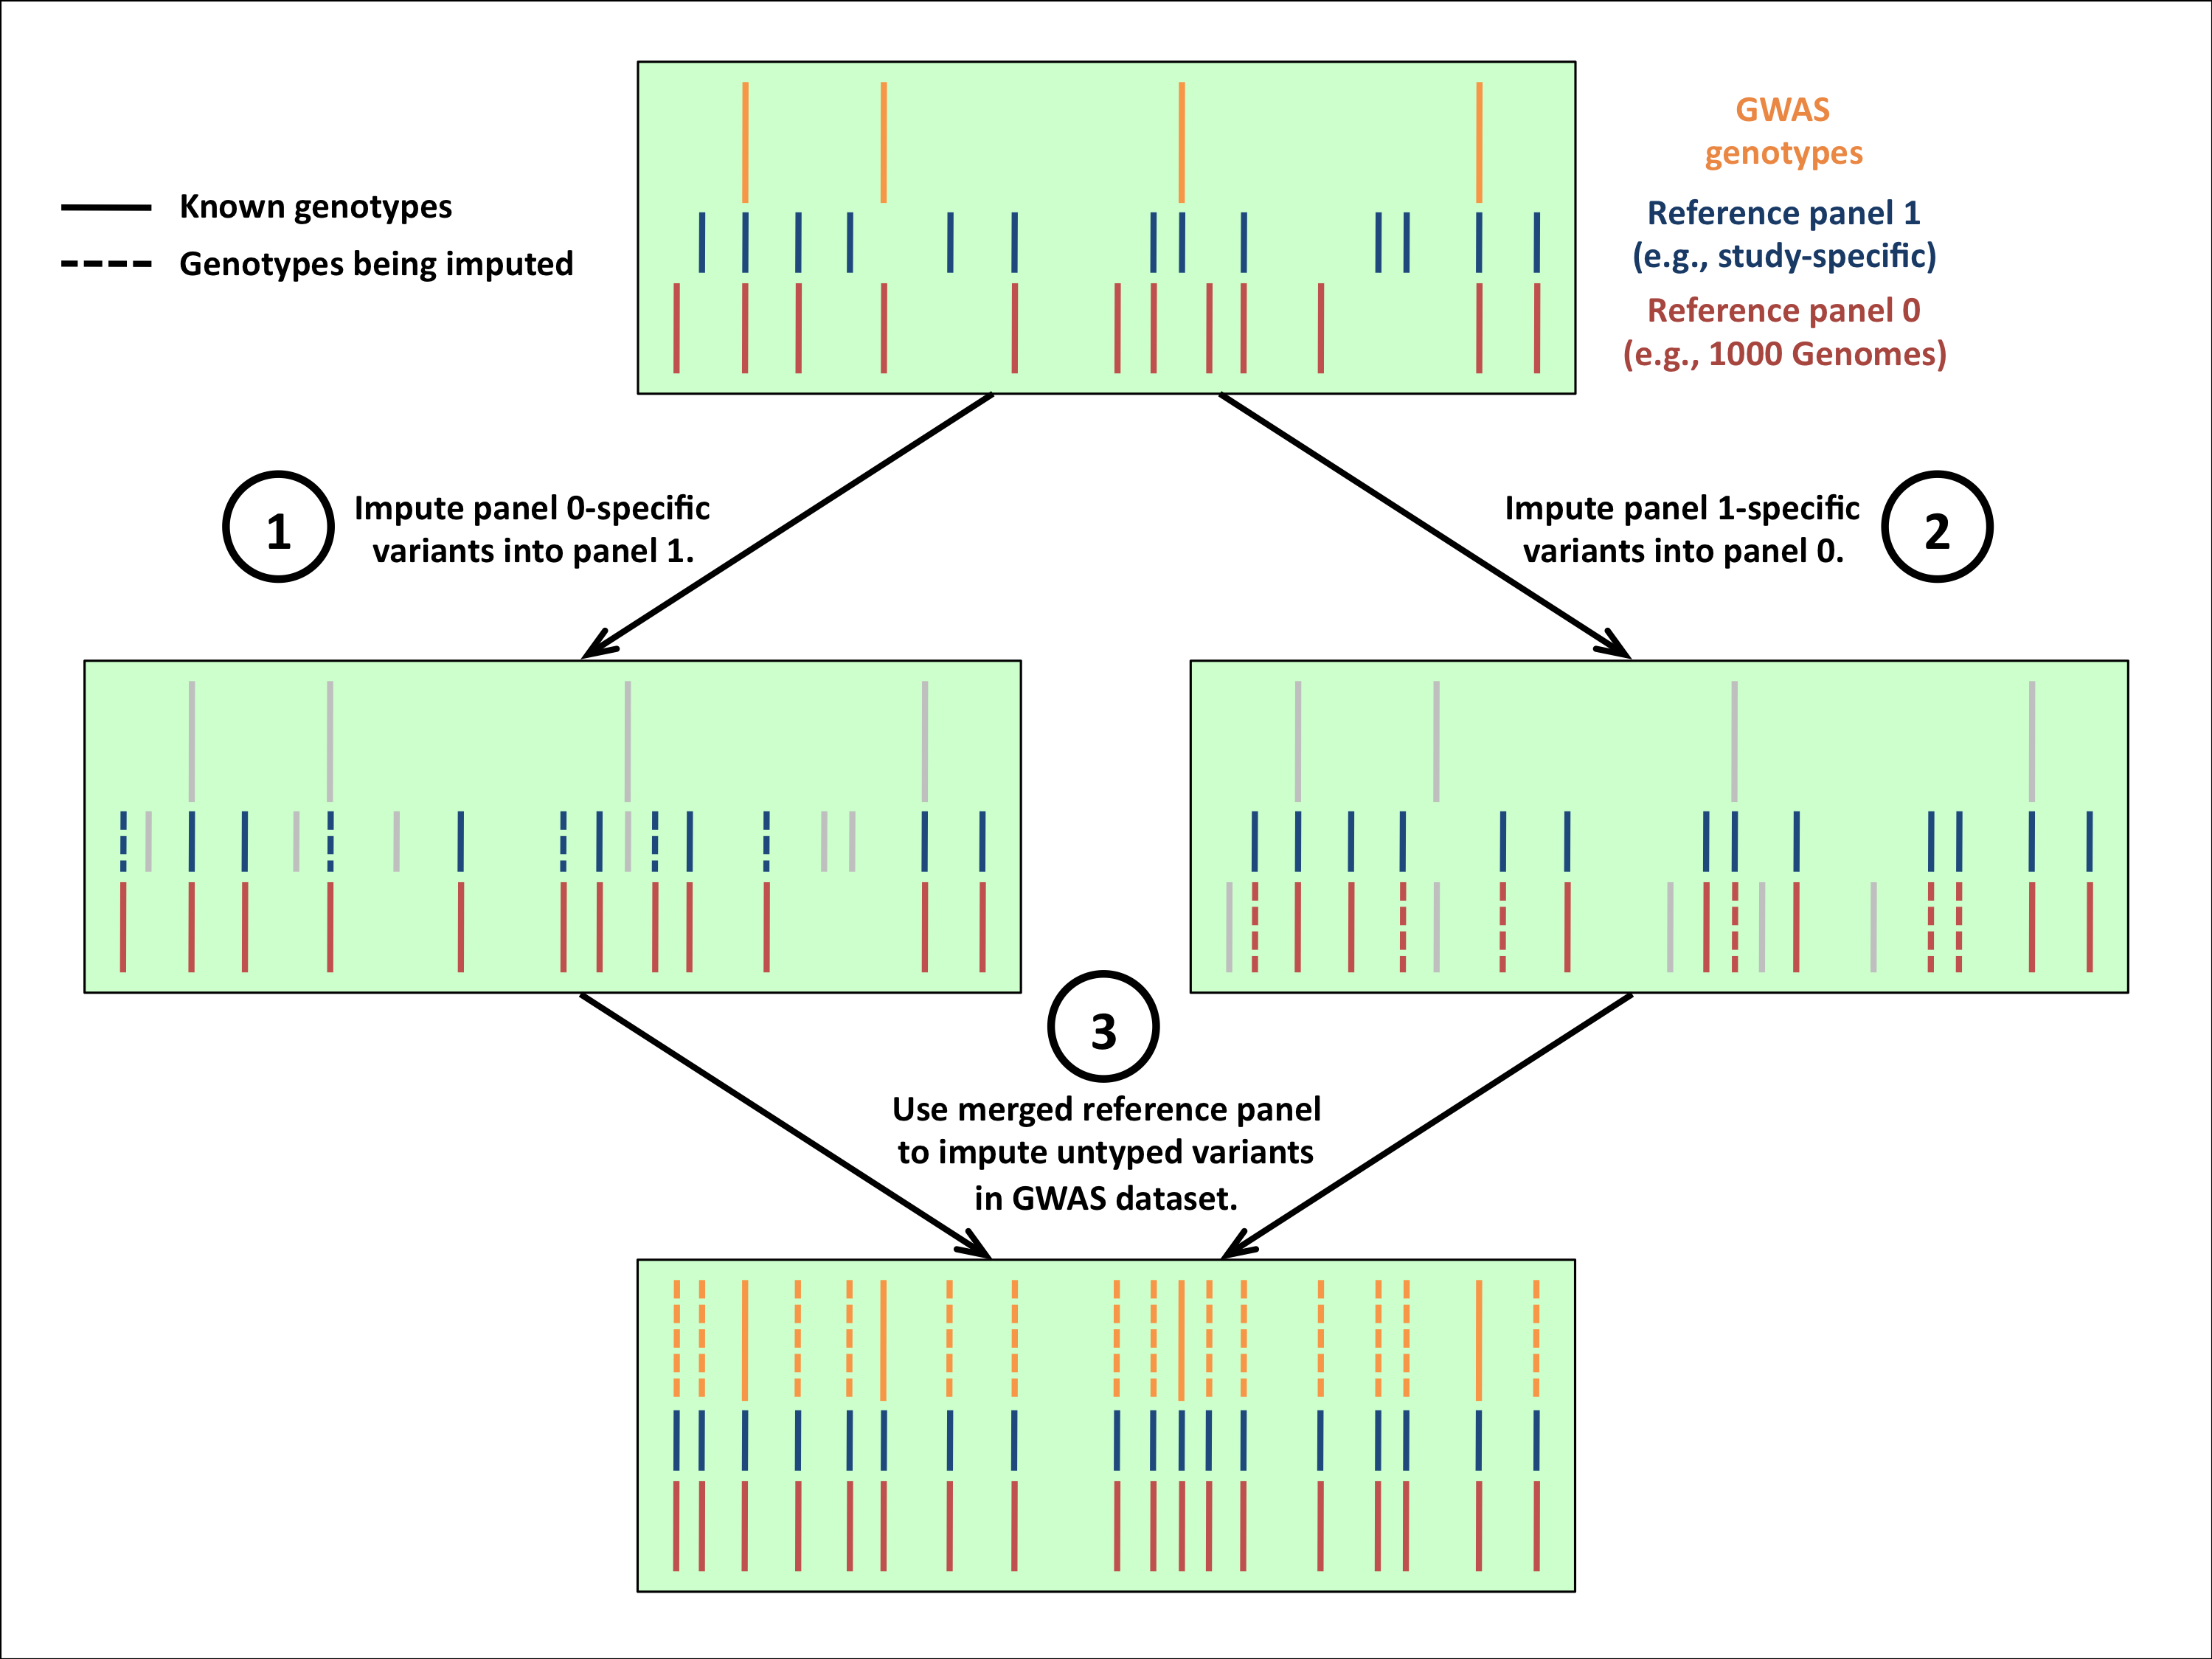
\includegraphics[width=0.6\textwidth]{merging_reference_panels}
\caption{The principle of creating a non-sparse matrix is the same as the merger of reference panels by imputation software. Figure copied from \href{http://mathgen.stats.ox.ac.uk/impute/merging\_reference\_panels.png}{IMPUTE2 web site}.}
\label{fig:merging_reference_panels}
\end{figure}

\begin{figure}[!htbp]
\centering
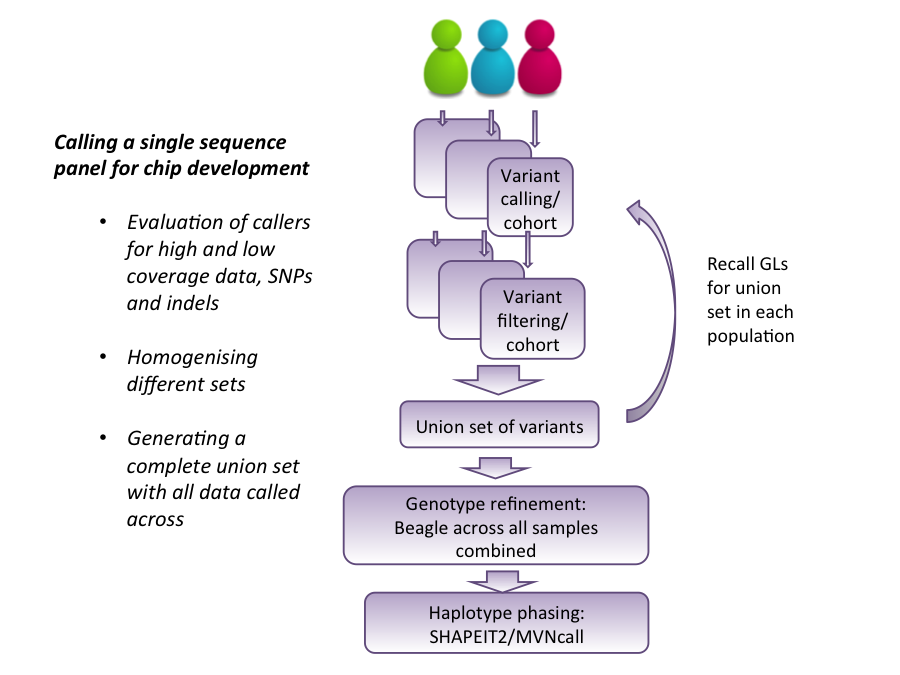
\includegraphics[width=0.8\textwidth]{calling}
\caption{Homogenised calling across all datasets to generate a single panel}
\label{fig:calling}
\end{figure}
